\documentclass[tikz,border=4pt]{standalone}
\usepackage{amsmath}
\usetikzlibrary{arrows.meta,calc}
\definecolor{ink}{HTML}{141518}
\definecolor{sub}{HTML}{525866}
\definecolor{cobalt}{HTML}{1D4ED8}
\begin{document}
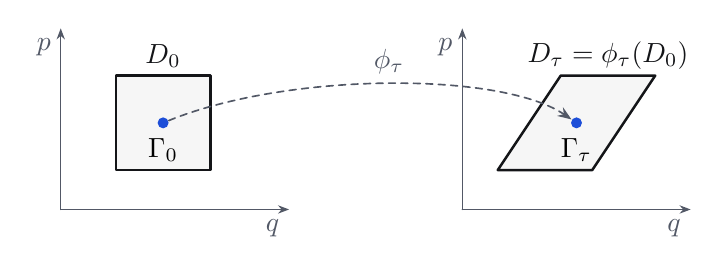
\begin{tikzpicture}[
    line cap=round, line join=round,
    axis/.style={-{Stealth[length=4pt]}, sub, line width=0.5pt},
    region/.style={ink, line width=0.9pt, fill=ink!4},
    pt/.style={circle, fill=cobalt, inner sep=1.4pt}
  ]
  % ---- 左：時刻 0 の位相空間 ----
  \begin{scope}
    \draw[axis] (0,0) -- (2.9,0) node[below left, sub] {$q$};
    \draw[axis] (0,0) -- (0,2.3) node[below left, sub] {$p$};
    \draw[region] (0.7,0.5) rectangle (1.9,1.7);
    \node[pt] (G0) at (1.3,1.1) {};
    \node[below=2pt] at (G0) {$\Gamma_0$};
    \node[ink] at (1.3,1.95) {$D_0$};
  \end{scope}
  % ---- 右：時刻 tau の位相空間（せん断しても面積は同じ） ----
  \begin{scope}[xshift=5.1cm]
    \draw[axis] (0,0) -- (2.9,0) node[below left, sub] {$q$};
    \draw[axis] (0,0) -- (0,2.3) node[below left, sub] {$p$};
    \draw[region] (0.45,0.5) -- (1.65,0.5) -- (2.45,1.7) -- (1.25,1.7) -- cycle;
    \node[pt] (Gt) at (1.45,1.1) {};
    \node[below=2pt] at (Gt) {$\Gamma_\tau$};
    \node[ink] at (1.85,1.95) {$D_\tau = \phi_\tau(D_0)$};
  \end{scope}
  % ---- 時間発展の写像 ----
  \draw[-{Stealth[length=5pt]}, sub, line width=0.6pt, dash pattern=on 2.5pt off 2pt]
    (G0) .. controls (2.9,1.75) and (5.6,1.75) .. node[above, sub] {$\phi_\tau$} (Gt);
\end{tikzpicture}
\end{document}
